\documentclass[sigconf]{acmart}
\settopmatter{printacmref=false} % Removes citation information below abstract
\renewcommand\footnotetextcopyrightpermission[1]{} % removes footnote with conference information in first column
\pagestyle{plain}
\usepackage{booktabs} % For formal tables
\usepackage{csquotes}

\begin{document}
\title{Inference of Discrete Ontologies}
\date{May 14, 2017}
\subtitle{11-727 Final Report}

\author{Ben Striner}
\email{bstriner@andrew.cmu.edu}


\begin{abstract}
Machine-understandable representations are not frequently human-understandable representations. A common method to attempt to understand dense representations is postmortem clustering of those representations into a structured discrete space such as a tree or ontology. It is especially desirable to learn discrete embeddings of semantic information because traditional semantic resources such as Wordnet and Propbank have tree-like structures. I compare the information content of dense embeddings to the information content of postmortem clustering of those embeddings. I also propose two methods for learning discrete embeddings that show improved performance compared to postmortem clustering. The proposed methods produce hierarchies with better predictive power than hierarchies produced by postmortem clustering, so should provide more meaningful clustering when applied to various semantic tasks. Comparisons between models are provided using a simple skipgram objective but architectures could be used to place a discrete, structured bottleneck into any neural network. Clustering methods do not adequately capture the information contained in a dense embedding and additional architectures are required to represent information in a structured discrete space. Further analysis of the class of architectures that learn discrete structured embeddings would provide a tool to use for many semantic tasks.
\end{abstract}

\maketitle

\section{Introduction}

Semantic knowledge is traditionally represented in a structured discrete space. Linguistic knowledge is very naturally represented using trees or networks. Exemplary ontologies include Wordnet, Penman Upper Model,  Dublin Core, OpenCyc, Freebase, and DBpedia. There are many differences between the ontologies but a common trait is some sort of symbolic tree or network structure. An ontology typically contains some sort of symbol set and some set of rules and relationships.

The natural way to encode information and rules in a neural network are dense activations and dense weights. However, human beings find it hard to understand or visualize dense embeddings so clustering or dimensionality reduction is used to make those embeddings understandable. It is very common in natural language processing to report various clusterings and visualizations of dense representations. I will collectively refer to methods of analyzing a dense embedding after training as postmortem methods.

I experimentally compared postmortem methods that impose structure on a dense embedding to methods that directly learn a structured representation. I found that learning structured representations provided higher-quality representations than postmortem methods. I compared methods using a skipgram objective but techniques could be applied to other tasks.

None of the tested methods perfectly compress information into a limited structured discrete representation. Further analysis of architectures that learn discrete embeddings is required to build better tools to apply to semantic tasks.

It is not an unreasonable assumption that some distance measure or primary component analysis on a dense embedding is related to the information content. However, this is not a perfect relationship and structured methods can help identify what distinguishing features are important.

\section{Line in the Sand}

Conventional ontologies are  structured, discrete and deterministic. Some are trees but others are networks or partially-ordered.

A node's location in a tree can be represented as a sequential series of symbols representing each branch taken from the root node. For simplicity, experiments were performed using a simple binary tree with a depth of 10 but more complicated structures are possible. Learned embeddings represent at most 10 bits of information. The fixed tree depth and width makes computations more efficient.

The meaning of a word cannot be completely represented in a discrete fashion. Many semantic and linguistic phenomena are lines in the sand. There are many blurry edge cases but that does not undermine the usefulness of categories for most situations. An ideal ontology should have the properties of being mostly discrete and deterministic while still allowing for some ambiguous or edge cases.

Human beings can both identify members of a category (a discrete task) and identify certain members as more or less prototypical (a continuous task).

The proposed models can be easily viewed as discrete trees by using $\operatorname{argmax}$ but are actually differentiable approximations to a discrete tree. This enables use of the embeddings as both a continuous differentiable value and a discrete value.

\section{Related Work}

This paper uses a simple skipgram objective to compare representation learning between several architectures. Word representations learned from simple models have been found to encode some amount of semantic information. \cite{DBLP:journals/corr/MikolovSCCD13} \cite{DBLP:journals/corr/abs-1301-3781}

More advanced objectives would cause different, possibly more useful, information to be learned. For example, dependency-based word embeddings provide an objective with arguably more semantics than a skipgram. \cite{Levy2014}

Word representations can be factored using matrix decomposition but here I focus on neural methods. \cite{pennington2014glove}

Word ontologies have been embedded into dense vectors, the inverse of the current task. \cite{Bordes:2011:LSE:2900423.2900470}

There exists a great deal of work related to sub-word embeddings, such as \cite{Li2015}, that could be combined with the current work.

Deep structured semantic model (DSSM) provides a continuous structured representation of semantics \cite{unsupervised-learning-of-word-semantic-embedding-using-the-deep-structured-semantic-model}. 

There are many improvements to the simple softmax. Hierarchical softmax \cite{Morin05hierarchicalprobabilistic} and negative sampling provide significant performance improvements. I used a vanilla softmax with uniform smoothing to ensure a simple and fair comparison between models.

SeqGAN provides a method for discrete inference using reinforcement learning techniques \cite{DBLP:journals/corr/YuZWY16}. Experiments in the current paper relate to differentiable approximations to discrete inference, as actual discrete inference requires RL or other methods. However, it may be the case that some types of inference can only be performed using RL methods.

\section{Baseline Models}

I trained two baseline models to estimate the upper and lower bounds of performance on the skipgram objective with regard to the information content of the encodings. An unconstrained skipgram model estimates an upper bound on performance given a context word. A unigram model estimates a lower bound on performance given no context.

\subsection{Skipgram Model}

I trained a skipgram model with an unconstrained dense hidden representation. The model consists of an embedding $z$ of input word $x$ and an MLP $f$ with softmax activation. 
The loss is $-\log( f_y(z))$ where $y$ is a word sampled from the context of $x$.

This baseline representation estimates the maximal unconstrained information content of an embedding for the skipgram objective.

\subsection{Unigram Model}

I trained a unigram model to predict words $y$ without $x$ as a given. This model estimates the performance of a skipgram model if the embedding encoded no information at all.

\section{Structured Discrete Models}

I compared two general approaches to learning structured discrete representations. Learned embeddings from different approaches were compared using the same validation model.

\begin{itemize}
\item Learn an unstructured representation and perform postmortem clustering
\item Learn a structured or constrained representation that clusters easily
\end{itemize}

\subsection{Validation Model Architecture}

The goal of this paper is to compare several methods for generating sequential discrete embeddings. Each embedding is validated on the same model to provide a fair comparison between methods.

The input word $x$, from a set of cardinality $k_x$, is embedded as $z$, a sequence of discrete symbols from a set of cardinality $k_z$. The embedding matrix is the discrete output of one of the discussed methods and is not trained during validation.

A recurrent network using residual units creates cumulative representations of the discrete symbols, $h_{i+1} = h_i + f(h_i, z_i)$. Each hidden representation encodes information about all of the previous symbols.

A multi-layer network predicts a $y$ sampled from the context window of $x$. This network is distributed over the depth of $h$. The loss is sum of the predicted negative log likelihood of $y$ over the depth of $h$.

The model does not predict a single probability but a series of probabilities given cumulative amounts of $z$. This allows for an analysis of how information is distributed sequentially over each symbol in $z$.

\subsection{Postmortem Clustering}

I experimented with two postmortem clustering methods, one top-down and one bottom-up.

\begin{itemize}
\item As a top-down method, I iteratively constructed a hierarchy of Gaussian Mixture Models as in \cite{Mnih:2008:SHD:2981780.2981915}. 
\item As a bottom-up method I used agglomerative binary clustering.
\end{itemize}

For both methods, I clustered dense embeddings learned by the baseline skipgram model. I clustered into a binary tree truncated to a depth of 10. These embeddings contain exactly 10 bits of information.

I then trained a validation model to predict samples drawn from a context window based only on the discrete embedding, to determine how much information was preserved by clustering.

\section{Learning Structured Representations}

Traditional ontologies are structured, discrete, and deterministic. Direct inference of a hidden representation that is discrete and deterministic requires reinforcement learning, expectation-maximization, or other methods because a simple approach is not differentiable. While not completely infeasible, I discuss models that approximate discrete deterministic inference while maintaining differentiability.

\begin{itemize}
\item A softmax output can be interpreted as representing a deterministic continuous value that approximates a one-hot encoding.
\item A softmax output can also be interpreted as representing stochastic probabilities over a discrete value.
\end{itemize}

These two interpretations of softmax lead to two approaches to approximate a discrete, structured, deterministic embedding.

\subsection{Deterministic Model}

The simpler of the two proposed models interprets the hidden representation as a deterministic continuous approximation to a one-hot encoding. Model input $x$ is embedded using a matrix of shape $(\text{tree depth}, z_k)$ and a softmax is applied over the last dimension. This results in $z$, a series of softmax encodings for each input $x$.

A recurrent network with residual units builds a cumulative representation $h$ of the embedding $z$. A multi-layer network predicts $y$ based on each $h$.

The loss is the sum of the negative log likelihoods given each cumulative amount of $z$.

An adversary regularizes the softmax encoding of $z$ towards saturation.

The embedding approximates a one-hot encoding but an infinite amount of information could hypothetically be encoded into only one dimension. Regularization and the softmax provide a bottleneck and reduce the amount of information that can flow but it is a soft limit that depends on many factors.

Transformation from learned $z$ to a sequential discrete deterministic embedding is just an argmax over the last axis.

\subsection{Stochastic Model}

The more complex of the two proposed models interprets the hidden representation as a distribution over possible discrete encodings. As before, input $x$ is embedded using a matrix of shape $(\text{tree depth}, z_k)$ and a softmax is applied over the last dimension to produce $z$, a sequence of discrete distributions.

A recurrent network with residual units builds a cumulative representation $h$ of samples taken from $z$.

A prediction network outputs the negative log likelihood of $y$ given each possible $z_i$ and the previous $h$. The loss of the model is the sum of the loss given each possible $z_i$ times the probability of that $z_i$. This unit is repeated for the depth of the network.

$$ loss = \sum_z-P(z \mid x) \log P(y \mid z)$$

An adversary regularizes the softmax $z$ towards saturation.

The prediction network is capable of exactly $k_z$ distributions at each step. $z$ represents a probabilistic choice between those distributions at each step and bottlenecks the information to a choice over exactly 1 bit of information if $z_k=2$.

Transformation from learned $z$ to a sequential discrete deterministic embedding is again just an argmax over the last axis.

\subsection{Adversarial Regularization}

A form of adversarial regularization was used to encourage the softmax embedding to saturate. The goals are twofold.

\begin{itemize}
\item Minimize divergence between uninformed prior and encodings marginalized over words
\item Maximize divergence between uninformed prior and encodings conditional on words
\end{itemize}

Such regularization is trivial given a depth of one but given multiple layers marginalization over words given partial embeddings becomes increasingly difficult. 

A solution is to use an adversary that attempts to learn the marginal distribution given partial embeddings.
A network is trained to predict $P(z_i \mid z_{i-1} \ldots z_0)$, the distribution of $z$ marginalized over words.
The skipgram model is then regularized to maximize $D( P(z_i \mid z_{i-1} \ldots z_0) \mid \mid P(z_i \mid x, z_{i-1} \ldots z_0))$, 
the divergence between the marginal and the conditional distributions.

I tested several measures and metrics such as KL divergence and found that Earth Mover / Wasserstein distance appeared to work the best.

\section{Results}

I trained each architecture on the Brown corpus. I used a simple corpus and simple skipgram objective so I could quickly train and compare all 8 models but methods could be applied to more interesting objectives.

The unigram and skipgram models provided upper and lower bounds on performance as expected. These bounds on NLL were 5.56 and 5.91 (see Table \ref{t:baseline}).

Postmortem GMM and agglomerative clustering show a significant performance gap between the skipgram model and the discretized embeddings, shown in Figure \ref{f:postmortem}.

Proposed discrete and stochastic methods also show a gap between the skipgram model and the discretized embeddings but the structured losses more closely resemble the discretized losses (see Figure \ref{f:proposed}).

The four discrete models are compared in Figure \ref{f:discrete} and Table \ref{t:discrete}.

The stochastic model was stopped early due to time constraints. The effect of this is that the model trained on the output of the stochastic model performed better than the stochastic model itself, if only for the first bit.

\begin{figure}
\caption{Postmortem Methods}
\label{f:postmortem}
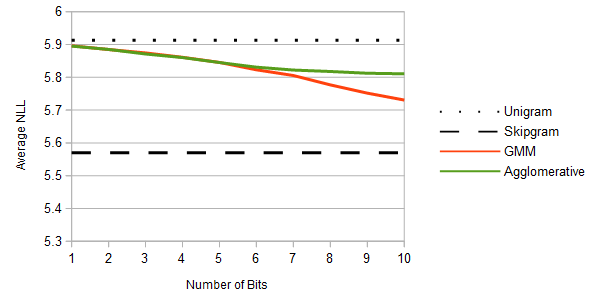
\includegraphics[scale=0.5]{images/postmortem.png}
\end{figure}

\begin{figure}
\caption{Proposed Methods}
\label{f:proposed}
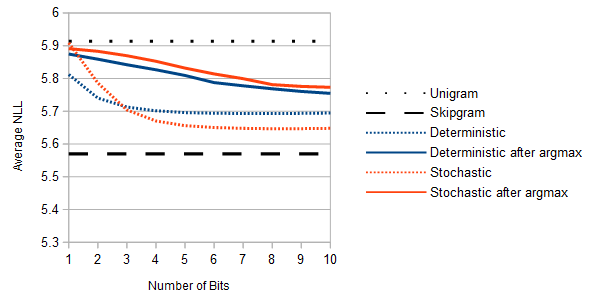
\includegraphics[scale=0.5]{images/proposed.png}
\end{figure}

\begin{figure}
\caption{Comparison of Discrete Embeddings}
\label{f:discrete}
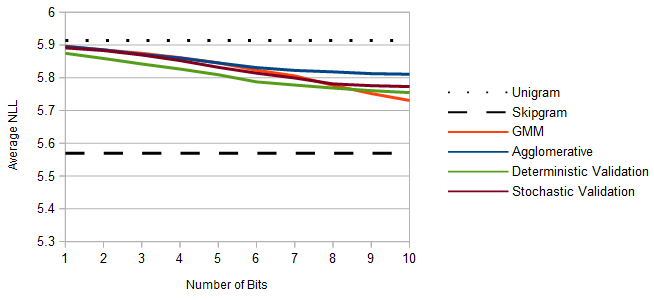
\includegraphics[scale=0.5]{images/discrete.png}
\end{figure}

\begin{table}
\caption{Skipgram and Unigram Models}
\label{t:baseline}
  \begin{tabular}{l r}
	\hline \hline
	 Model & Average NLL \\
	\hline
	Skipgram & 5.5699 \\
	Unigram & 5.9135 \\
	\hline \hline
  \end{tabular}
\end{table}

\begin{table}
\caption{Discrete Models}
\label{t:discrete}
  \begin{tabular}{l r r r}
	\hline \hline
 & \multicolumn{3}{|c|}{NLL} \\
	 Model & 1 bit & 5 bits & 10 bits\\
	\hline
GMM & 5.8964 & 5.8455 & 5.7308 \\
Agglomerative & 5.8954 & 5.8453 & 5.8108 \\
Deterministic & 5.8746 & 5.8092 & 5.7547 \\
Stochastic & 5.8913 & 5.8318 & 5.7731 \\
	\hline \hline
  \end{tabular}
\end{table}

\section{Discussion}

Agglomerative clustering is the least performant method of those tested. As experiments are designed to see how much information is contained in the top of the hierarchy, it is not unexpected that a bottom-up method performed poorly.

Both proposed models performed better than GMM on the early bits, but were outperformed by GMM by the tenth bit. If I had used fewer bits, proposed models would have outperformed GMM. A likely component of the explanation is that the proposed models use recursive networks with a depth of 10, and gradient and stability issues may contribute to the predictions after the first few bits.

Initial experiments seemed to work well with broader trees that would require less depth but I used binary trees for simplicity. Broader trees would help but not solve any issues associated with tree depth.

The GMM model is algorithmically constrained to a balanced tree. Proposed models are regularized towards a balanced tree but are not perfectly balanced, which may also contribute to the better early performance but worse late performance. Further experimentation regarding the adversarial regularization and analysis of how balanced the tree is would be useful.

Proposed models outperform GMM on the early bits, therefore postmortem clustering, at least the GMM implementation tested, does not maximally capture the information relevant to the objective at the highest levels of the hierarchy.

The discretization gap is the loss in performance between the continuous embedding and the discretized embedding. Discretization of the dense model requires clustering while discretization of proposed models is simply an argmax. As expected, the discretization gap is much greater between the dense model and clustering of the dense model than between the proposed models and the argmax of proposed models, although all experiments showed a large discretization gap.

The stochastic model showed a slightly smaller discretization gap than the discrete model, which is expected as the stochastic model has a tighter bottleneck and should more closely approximate the deterministic discrete tree.

Trained hierarchies were found to perform better on the objective function than hierarchies generated by clustering (at least at the upper levels of the hierarchy). Improved performance should lead to more meaningful and understandable hierarchies.

\section{Exploration}

Results indicate that trained hierarchies represent information related to the objective function better than clustering. If the skipgram objective requires some semantic information, this implies that learned hierarchies better represent semantics than postmortem clustering. This cannot be easily quantified and is only true to the extent that the objective in question actually requires semantic information.

With that in mind, there are semantic relationships in the learned ontology. There are also many leaves that defy explanation. With better objectives and better methods, the goal is to learn a semantic hierarchy akin to Wordnet or Propbank.

An exemplary learned relationship is that between pronouns as depicted in Figure \ref{f:pronouns}. First and second person pronouns are one branch away from third person pronouns, and two branches away from pronoun contractions.

\begin{figure}
\caption{Learned pronoun relationships}
\label{f:pronouns}
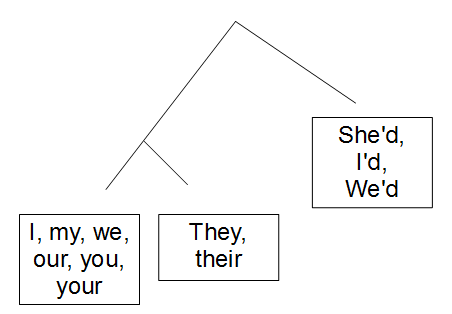
\includegraphics[scale=0.5]{images/pronouns.png}
\end{figure}

Some categories are large but still seem to capture something. For example, one category contains 108 terms related to banking such ``adjustment'', ``allotment'' and ``antitrust'' to ``taxes'', ``treasury'' and ``welfare''.

Smaller categories appear to be more specific. For example, one leaf contains only two terms, ``Christianity'' and ``Protestant''. 

``Inches'' and ``minutes'' are in the same leaf, one branch away from ``years'' and cousins with ``centuries'', ``weeks'' and ``decades''. These are all second-cousins with a leaf containing 10 terms including ``hundred'', ``billion'', ``million'', ``dollars'', ``cents'', ``tons'', ``acres'' and ``Lb''.

\section{Language Modeling Results}

I also trained embeddings on a neural language model to hopefully generate more meaningful embeddings than those learned by a simple skipgram. However, as a full language model takes a lot longer to train than a skipgram, it was not feasible to train and compare 8 language models over the course of a semester even on a small dataset like Brown.

I also experimented with wider networks which appeared to make training slightly easier.

Based on initial experimentation, language models appear to generate more interesting embeddings.

I trained a model so the middle word could be used to predict the context words from left to right. Following are some example contexts that the model generated from the middle word. The examples show that the encoding carries some combination of syntactic and semantic information.

\begin{displayquote}
 carrying the [suitcase] . there \\
a partisan [undertaking] when some \\
development of [residential] communities \\
our parents [winked] and muttered \\
they had [foreseen] the huge \\
trembling considerable [handicap] about her \\
the west [indies] all the
\end{displayquote}

The language model learned some meaningful categories. For instance, some inferred groupings:
\begin{itemize}
\item waiter and bartender
\item Sox and Yankees
\item hip and knee
\end{itemize}

The language model also learned some relationships over the structure of the model. For example, ``murderer'', ``attacker'', ``brute'' and ``army'' are all separated by one branch.

\section{Future Work}

I present analysis of extreme dimensionality reduction, compressing embeddings to a sequence of a few bits. Further analysis of methods for embedding into a discrete space would enable new models for language and other processing.

Reduction to a discrete space is especially important for linguistics since so many phenomena are naturally described in terms of symbols.

The discrete embedding model could be expanded to perform various types of beam searching and backtracking. Although that would make the implementation difficult it could be engineered to more closely embody theories of reasoning. The current implementation is not ideal and could be expanded into a much more powerful approach.

The present model is not trained to distinguish word senses. Inference of discrete choices, such as word senses, is an important aspect of future work

More challenging will be inference of a rule set. Future work should strive to infer a symbol set and rule set that can be used for higher-level logic.

Current models could be improved by analyzing issues with recurrence and balancing the model to improve performance for the deeper bits.

It would also be useful to compare proposed models using more challenging objectives than a skipgram.

Experiments used a simple binary tree for simplicity and consistency with prior work. More complicated trees, networks, or partially-ordered trees could provide more expressive hidden representations.

It would also be valuable to compare performance on learned trees to those based on coding theory such as a Huffman tree.

The task of efficient inference of discrete structured hidden representations will not be easy, as shown by the large discretization gaps across experiments.

Further analysis should also include determining whether an example is prototypical, which could be operationalized by the amount of saturation of the softmax. Viewing all words in an ontology may be overwhelming but filtering for the most prototypical words could make it manageable.

\section{Implementation Details}

Preprocessing consisted of removing punctuation and non-ASCII symbols, down-casing, and replacing words that occur less that 20 times with an unknown symbol.

All discrete models used a depth of 10 and symbol set of 2, so represent a total of 10 bits of information per word. After filtration and cleaning the corpus consisted of 4908 unique words plus the unknown symbol, so there should be an average of $\frac{4909}{2^{10}} \approx 4.8$ words per encoding.

Softmax activations in the prediction layers were uniformly smoothed by a factor of $10^{-8}$ to avoid numerical instability.

Recursive portions of the model were built using residual units \cite{DBLP:journals/corr/HeZRS15} in which each unit learns only a residual change to the hidden state,
$h_{i+1} = h_i + f(h_i, x_i)$ where $f$ is a multilayer network.

Models used LeakyReLU units for all internal activations \cite{Maas2013} \cite{DBLP:journals/corr/XuWCL15}.

A window of size 2 was used for context, providing a reasonable difference between the skipgram and unigram models. At large context sizes the performance of a skipgram model approaches a unigram model.

For further details, please refer to the source code, available on Github\footnote{\url{https://github.com/bstriner/discrete-skip-gram}}.

\nocite{*}

\bibliographystyle{ACM-Reference-Format}
\bibliography{bstriner_report} 

\end{document}
